\documentclass[12pt,a4paper]{article}

\usepackage[utf8]{inputenc}
\usepackage[english]{babel}
\usepackage{amsmath}
\usepackage{amsfonts}
\usepackage{amssymb}
\usepackage{makeidx}
\usepackage{graphicx}
\usepackage{subcaption}
\usepackage{caption}
\usepackage{float}
\usepackage[left=2cm,right=2cm,top=2cm,bottom=2cm]{geometry}
\usepackage{tikz}
\usepackage{pdfpages}
\pagestyle{plain}
\usepackage{bm}
\usepackage{ulem}
\usepackage{units}
\usepackage{makecell}

%Kopf und Fußzeile:
\usepackage{fancyhdr}
\pagestyle{fancy}
\fancyhf{}
\renewcommand{\footrulewidth}{0.4pt}
\usepackage{array}   % for \newcolumntype macro
\newcolumntype{C}{>{$}c<{$}} % math-mode version of "c" column type

\fancyhead[L]{Computational photonics}
%\fancyhead[C]{Dr. Bj\"orn Leder}
\fancyhead[R]{Excercise 3}
\fancyfoot[L]{\today}
\fancyfoot[R]{page \thepage}
\fancyfoot[C]{Julien Kluge}

% Code-Listings
\usepackage{listings}
\lstset{
language=c,
showstringspaces=false,
numbers=left,
xleftmargin=2em}

% Ganze Dateien als Verbatim einbinden
%\usepackage{verbatimfiles} % downloaded from ctan.org

\title{Computational photonics}
\author{Julien Kluge}
\date{\today}

%============================================================
% Dokument
%============================================================
\begin{document}

\lstset{numbers=left}

\begin{center}
\large{\textbf{Computational photonics -- Excercise 3}} \\
~\\
\small{-- Julien Kluge (564513) --}\\
~\\
Date: \today
\end{center}
\hrule
	\section*{1)}
	A picture of the Gerthsen wall was fourier transformed with an
	fft shift applied. THe following images where acquired: 
	\begin{figure}[H]
		\begin{subfigure}[b]{0.48\textwidth}
			\centering
			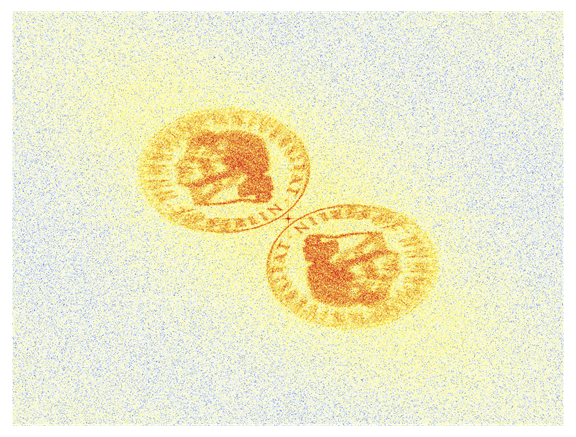
\includegraphics[width=\textwidth]{Fourier.png}
			\caption{Full section transform.}
		\end{subfigure}
		\begin{subfigure}[b]{0.48\textwidth}
			\centering
			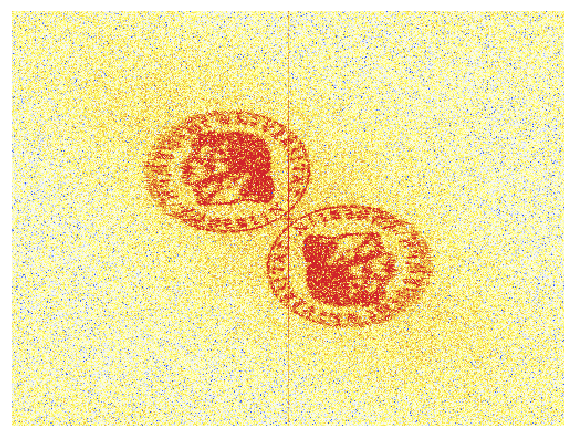
\includegraphics[width=\textwidth]{Fourier_Cropped.png}
			\caption{Quarter section transform.}
		\end{subfigure}
		\caption{Image (a) used the whole image to perform the
		reverse transformation whereas (b) only left the left
		upper quadrant.}
	\end{figure}
	It can easily be seen, that a reduction of the region to
	transform on does not limit the size of the hu logo in the
	frequency domain but the sampling. Therefore the relative
	noise was increased.\\
	The image appears twice, since it was transformed from a
	real valued image. Therefore the phase was lost in encoding.
	This forces the image to apear twice.
\end{document}
